\section{Experimental Results}

\subsection{Generate Merkle tree}
\begin{frame}<beamer>
    \frametitle{Outline}
    \tableofcontents[currentsubsection]
\end{frame}

\begin{frame}{Experimental Results}
	\begin{table}[]
		\scriptsize
		\centering
		\begin{tabular}{crcc}
			  & Size    & File  & Directory \\
			  &			&		&		    \\
			A & 777 MB  & 48    & 6         \\
			B & 145 MB  & 54198 & 188       \\
			C & 5.95 GB & 45089 & 1459      \\
		\end{tabular}
        ~\\
        ~\\
        ~\\
		\caption{GENERATE MERKLE TREE'S TIME (IN SEC.)}
		\begin{tabular}{|c|c|c|r|}
			\hline
              & Non Hashed & Pre Hashed & Merkle tree Size \\ \hline
            A & 9.406    & 0.003    & 5.4 KB           \\ \hline
            B & 55.147   & 2.703    & 5.08 MB          \\ \hline
            C & 339.181  & 0.334    & 4.37 MB          \\ \hline
		\end{tabular}
        ~\\
        ~\\
        ~\\
        \caption{SERIALIZE \& DESERIALIZE MERKLE TREE OBJECT'S TIME (IN SEC.)}
		\begin{tabular}{|c|c|c|}
            \hline
              & Serialize & Deserialize \\ \hline
            A & 0.040      & 0.009       \\ \hline
            B & 0.756      & 0.299       \\ \hline
            C & 0.670      & 0.295       \\ \hline
		\end{tabular}
	\end{table}
\end{frame}

\subsection{Non POV}
\begin{frame}<beamer>
    \frametitle{Outline}
    \tableofcontents[currentsubsection]
\end{frame}

\begin{frame}{Experimental Results}{Non POV}
	\textcolor{blue}{not in the same network segment: from lab to my home (16 hops.)}\\
    \tiny
    \begin{table}[]
        \centering
        \begin{minipage}[c]{0.5\textwidth}
            \caption{The client device and SP are in the \newline same network segment}
            \begin{tabular}{lcc}
                                 & Upload (sec.) & Download (sec.) \\ \hline
                \textless 10 KB  & 0.010      & 0.007        \\ \hline
                \textless 100 KB & 0.014      & 0.013        \\ \hline
                \textless 1 MB   & 0.090      & 0.088        \\ \hline
                \textless 10 MB  & 0.367      & 0.354        \\ \hline
            \end{tabular}
            \begin{center}
                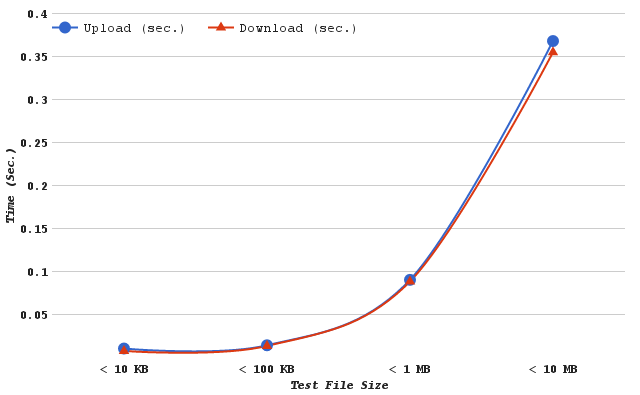
\includegraphics[width=\textwidth]{non_pov_same}
            \end{center}
        \end{minipage}%
        \begin{minipage}[c]{0.5\textwidth}
            \caption{The client device and SP are \alert{not} in the \newline same network segment}
            \begin{tabular}{lcc}
                                 & Upload (sec.) & Download (sec.) \\ \hline
                \textless 10 KB  & 0.069      & 0.056        \\ \hline
                \textless 100 KB & 0.121      & 0.087        \\ \hline
                \textless 1 MB   & 0.343      & 0.225        \\ \hline
                \textless 10 MB  & 1.675      & 0.699        \\ \hline
            \end{tabular}
            \begin{center}
                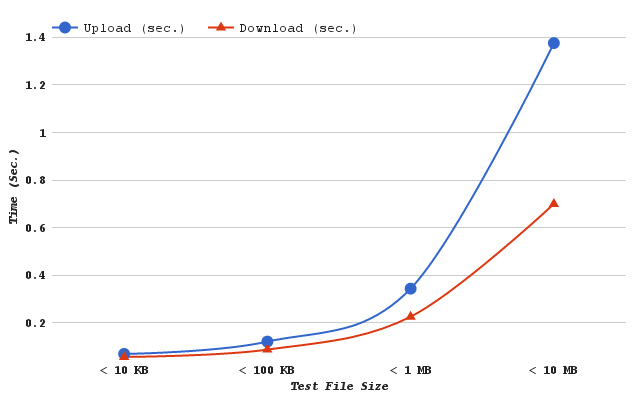
\includegraphics[width=\textwidth]{non_pov_not_same}
            \end{center}
        \end{minipage}
    \end{table}
\end{frame}

\subsection{Same Network Segment}
\begin{frame}<beamer>
    \frametitle{Outline}
    \tableofcontents[currentsubsection]
\end{frame}

\begin{frame}{Experimental Results}
{The client device and SP are in the same network segment - My Method}
	\scriptsize
    \begin{table}[]
    \centering
    \caption{THE EXECUTION TIME OF \alert{UPLOAD} OPERATIONS (IN SEC.) (Account C)}
    \begin{tabular}{lcccc}
                         & 3 Server & 5 Server & 7 Server & 9 Server \\ \hline
        \textless 10 KB  & 0.046 & 0.067 & 0.101 & 0.108 \\ \hline
        \textless 100 KB & 0.070 & 0.083 & 0.112 & 0.145 \\ \hline
        \textless 1 MB   & 0.153 & 0.166 & 0.200 & 0.203 \\ \hline
        \textless 10 MB  & 0.430 & 0.513 & 0.684 & 0.694 \\ \hline
    \end{tabular}
    \end{table}
    \begin{center}
		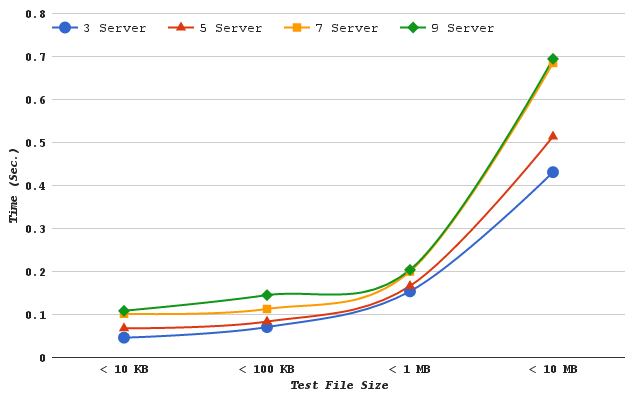
\includegraphics[width=.6\textwidth]{my_upload_same}
    \end{center}
\end{frame}

\begin{frame}{Experimental Results}
{The client device and SP are in the same network segment - My Method}
	\scriptsize
    \begin{table}[]
    \centering
    \caption{THE EXECUTION TIME OF \alert{DOWNLOAD} OPERATIONS (IN SEC.) (Account C)}
    \begin{tabular}{lcccc}
                         & 3 Server & 5 Server & 7 Server & 9 Server \\ \hline
        \textless 10 KB  & 0.042 & 0.054 & 0.064 & 0.078 \\ \hline
        \textless 100 KB & 0.053 & 0.055 & 0.083 & 0.097 \\ \hline
        \textless 1 MB   & 0.146 & 0.159 & 0.195 & 0.202 \\ \hline
        \textless 10 MB  & 0.392 & 0.476 & 0.622 & 0.625 \\ \hline
    \end{tabular}
    \end{table}
    \begin{center}
		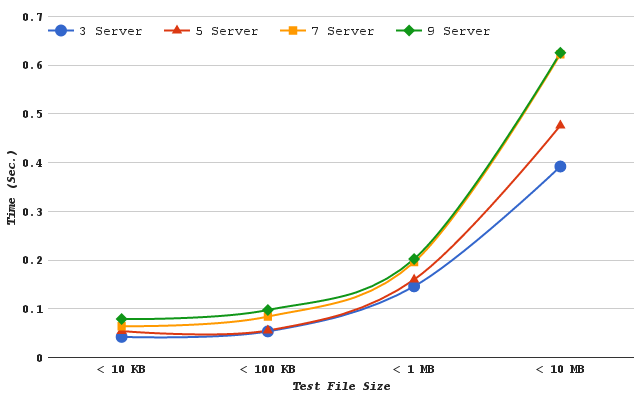
\includegraphics[width=.6\textwidth]{my_download_same}
    \end{center}
\end{frame}

\begin{frame}{Experimental Results}
{The client device and SP are in the same network segment - 2014 Cloud Com}
	\scriptsize
    \begin{table}[]
    \centering
    \caption{THE EXECUTION TIME OF \alert{UPLOAD} OPERATIONS (IN SEC.) (Account C)}
    \begin{tabular}{lccccl}
                         & sync 2   & sync 10  & sync 50  & sync 100 & sync 500 \\ \hline
        \textless 10 KB  & 0.146 & 0.184 & 0.332 & 0.409 & 0.760  \\ \hline
        \textless 100 KB & 0.194 & 0.209 & 0.341 & 0.491 & 0.932  \\ \hline
        \textless 1 MB   & 0.331 & 0.385 & 0.403 & 0.537 & 1.198  \\ \hline
        \textless 10 MB  & 0.501 & 0.518 & 0.576 & 0.819 & 1.242  \\ \hline
    \end{tabular}
    \end{table}
    \begin{center}
		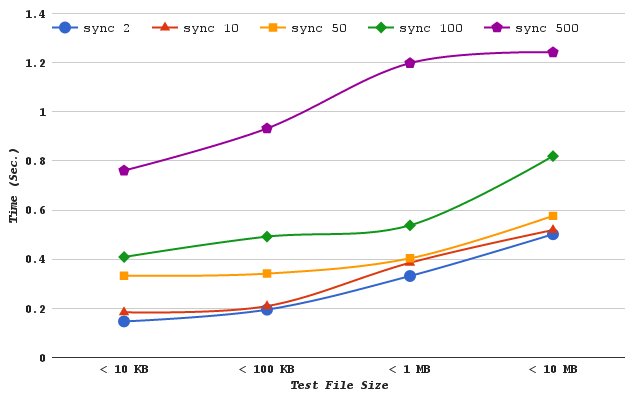
\includegraphics[width=.6\textwidth]{2014_upload_same}
    \end{center}
\end{frame}

\begin{frame}{Experimental Results}
{The client device and SP are in the same network segment - 2014 Cloud Com}
	\scriptsize
    \begin{table}[]
    \centering
    \caption{THE EXECUTION TIME OF \alert{DOWNLOAD} OPERATIONS (IN SEC.) (Account C)}
    \begin{tabular}{lccccl}
                         & sync 2   & sync 10  & sync 50  & sync 100 & sync 500  \\ \hline
        \textless 10 KB  & 0.121 & 0.249 & 0.331 & 0.515 & 1.675  \\ \hline
        \textless 100 KB & 0.134 & 0.258 & 0.338 & 0.564 & 1.796  \\ \hline
        \textless 1 MB   & 0.279 & 0.302 & 0.440 & 0.588 & 1.994  \\ \hline
        \textless 10 MB  & 0.462 & 0.539 & 0.595 & 1.171 & 2.241  \\ \hline
    \end{tabular}
    \end{table}
    \begin{center}
		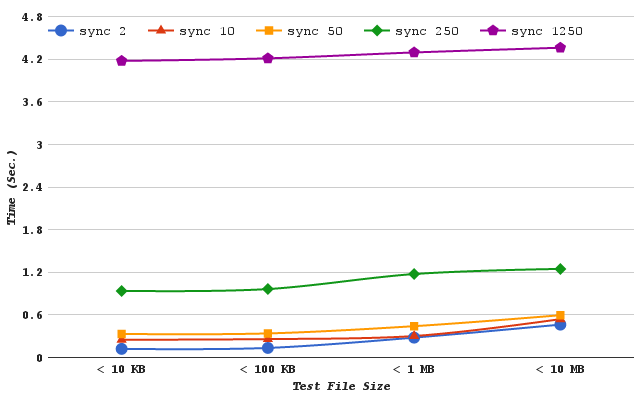
\includegraphics[width=.6\textwidth]{2014_download_same}
    \end{center}
\end{frame}

\begin{frame}{Experimental Results}
{The client device and SP are in the same network segment - UPLOAD operation}
	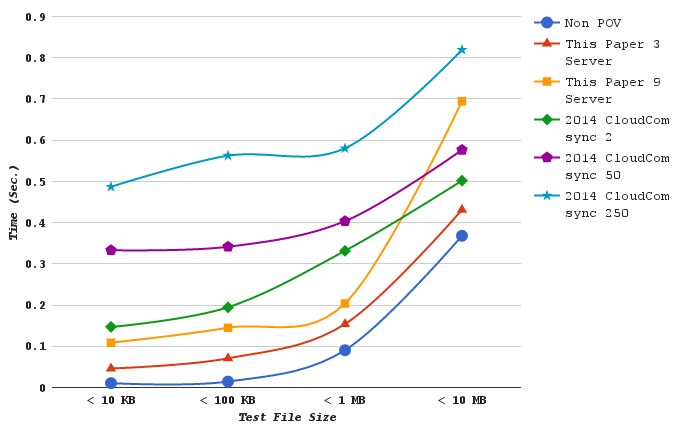
\includegraphics[width=\textwidth]{all_upload_same}
\end{frame}

\begin{frame}{Experimental Results}
{The client device and SP are in the same network segment - DOWNLOAD operation}
	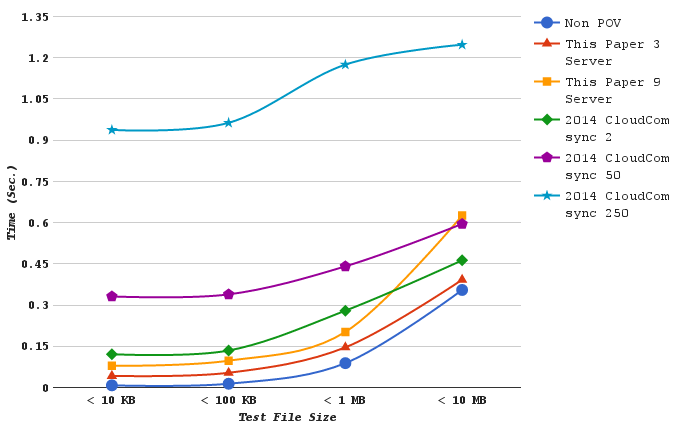
\includegraphics[width=\textwidth]{all_download_same}
\end{frame}

%TIMES
\begin{frame}{Experimental Results}
{The client device and SP are in the same network segment - UPLOAD Overhead}
	\scriptsize
    \begin{table}[]
    \centering
    \caption{My Method / Non POV (IN SEC.) (Account C)}
    \begin{tabular}{lcccc}
                         & 3 Server & 5 Server & 7 Server & 9 Server  \\ \hline
        \textless 10 KB  & 4.34 & 6.40 & 9.58 & 10.24 \\ \hline
        \textless 100 KB & 4.91 & 5.80 & 7.84 & 10.07 \\ \hline
        \textless 1 MB   & 1.70 & 1.83 & 2.21 & 2.25  \\ \hline
        \textless 10 MB  & 1.17 & 1.39 & 1.86 & 1.88  \\ \hline
    \end{tabular}
    \caption{2014 Cloud Com / Non POV (IN SEC.) (Account C)}
    \begin{tabular}{lccccl}
                         & sync 2    & sync 10   & sync 50   & sync 100 & sync 500 \\ \hline
        \textless 10 KB  & 13.83 & 17.35 & 31.39 & 38.55  & 71.72  \\ \hline
        \textless 100 KB & 13.52 & 14.52 & 23.72 & 34.18  & 64.75  \\ \hline
        \textless 1 MB   & 3.66  & 4.26  & 4.46  & 5.94   & 13.24  \\ \hline
        \textless 10 MB  & 1.36  & 1.40  & 1.56  & 2.22   & 3.37   \\ \hline
    \end{tabular}
    ~\\
    ~\\
    ~\\
    \alert{Avg: 3.97 times, Max: 6.99 times}
    \end{table}
\end{frame}

\begin{frame}{Experimental Results}
{The client device and SP are in the same network segment - DOWNLOAD Overhead}
	\scriptsize
    \begin{table}[]
    \centering
    \caption{My Method / Non POV (IN SEC.) (Account C)}
    \begin{tabular}{lcccc}
                         & 3 Server & 5 Server & 7 Server & 9 Server  \\ \hline
        \textless 10 KB  & 5.39 & 6.91 & 8.20 & 10.05 \\ \hline
        \textless 100 KB & 3.91 & 4.04 & 6.13 & 7.12  \\ \hline
        \textless 1 MB   & 1.64 & 1.80 & 2.21 & 2.28  \\ \hline
        \textless 10 MB  & 1.10 & 1.34 & 1.75 & 1.76  \\ \hline
    \end{tabular}
    \caption{2014 Cloud Com / Non POV (IN SEC.) (Account C)}
    \begin{tabular}{lccccl}
                         & sync 2    & sync 10   & sync 50   & sync 100   & sync 500  \\ \hline
        \textless 10 KB  & 15.45 & 31.84 & 42.23 & 119.48 & 532.25 \\ \hline
        \textless 100 KB & 9.82  & 18.89 & 24.74 & 70.34  & 307.57 \\ \hline
        \textless 1 MB   & 3.15  & 3.41  & 4.97  & 13.26  & 48.48  \\ \hline
        \textless 10 MB  & 1.30  & 1.52  & 1.67  & 3.51   & 12.28  \\ \hline
    \end{tabular}
    ~\\
    ~\\
    ~\\
    \alert{Avg: 7.91 times, Max: 21.24 times}
    \end{table}
\end{frame}

\subsection{Not Same Network Segment}
\begin{frame}<beamer>
    \frametitle{Outline}
    \tableofcontents[currentsubsection]
\end{frame}

\begin{frame}{Experimental Results}
{The client device and SP are \alert{not} in the same network segment - My Method}
	\scriptsize
    \begin{table}[]
    \centering
    \caption{THE EXECUTION TIME OF \alert{UPLOAD} OPERATIONS (IN SEC.) (Account C)}
    \begin{tabular}{lcccc}
                         & 3 Server & 5 Server & 7 Server & 9 Server \\ \hline
        \textless 10 KB  & 0.217 & 0.331 & 0.466 & 0.570 \\ \hline
        \textless 100 KB & 0.245 & 0.410 & 0.479 & 0.660 \\ \hline
        \textless 1 MB   & 0.433 & 0.594 & 0.640 & 0.786 \\ \hline
        \textless 10 MB  & 1.636 & 1.972 & 2.011 & 2.163 \\ \hline
    \end{tabular}
    \end{table}
    \begin{center}
		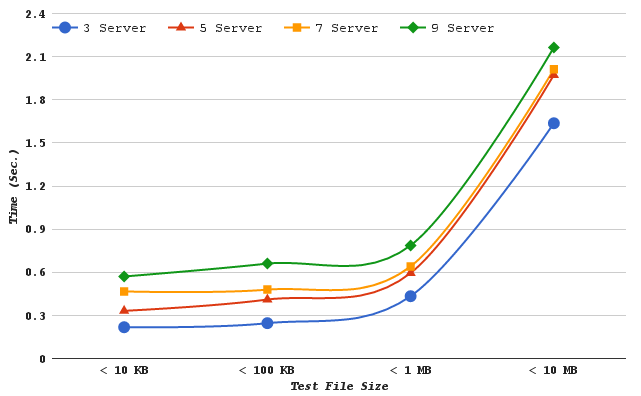
\includegraphics[width=.6\textwidth]{my_upload_not_same}
    \end{center}
\end{frame}

\begin{frame}{Experimental Results}
{The client device and SP are \alert{not} in the same network segment - My Method}
	\scriptsize
    \begin{table}[]
    \centering
    \caption{THE EXECUTION TIME OF \alert{DOWNLOAD} OPERATIONS (IN SEC.) (Account C)}
    \begin{tabular}{lcccc}
                         & 3 Server & 5 Server & 7 Server & 9 Server \\ \hline
        \textless 10 KB  & 0.263 & 0.358 & 0.490 & 0.556 \\ \hline
        \textless 100 KB & 0.270 & 0.396 & 0.567 & 0.597 \\ \hline
        \textless 1 MB   & 0.382 & 0.590 & 0.694 & 0.846 \\ \hline
        \textless 10 MB  & 0.823 & 1.086 & 1.208 & 1.278 \\ \hline
    \end{tabular}
    \end{table}
    \begin{center}
		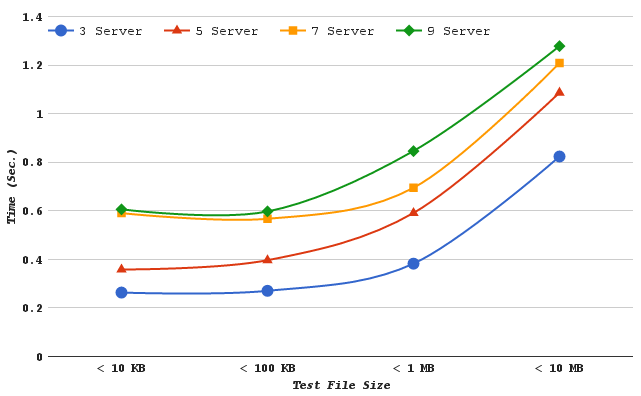
\includegraphics[width=.6\textwidth]{my_download_not_same}
    \end{center}
\end{frame}

\begin{frame}{Experimental Results}
{The client device and SP are \alert{not} in the same network segment - 2014 Cloud Com}
	\scriptsize
    \begin{table}[]
    \centering
    \caption{THE EXECUTION TIME OF \alert{UPLOAD} OPERATIONS (IN SEC.) (Account C)}
    \begin{tabular}{lccccl}
                         & sync 2   & sync 10  & sync 50  & sync 100 & sync 500  \\ \hline
        \textless 10 KB  & 0.362 & 0.411 & 0.486 & 0.500 & 1.227  \\ \hline
        \textless 100 KB & 0.377 & 0.416 & 0.508 & 0.563 & 1.375  \\ \hline
        \textless 1 MB   & 0.556 & 0.619 & 0.698 & 0.812 & 1.630  \\ \hline
        \textless 10 MB  & 1.525 & 1.882 & 1.929 & 1.962 & 2.753  \\ \hline
    \end{tabular}
    \end{table}
    \begin{center}
		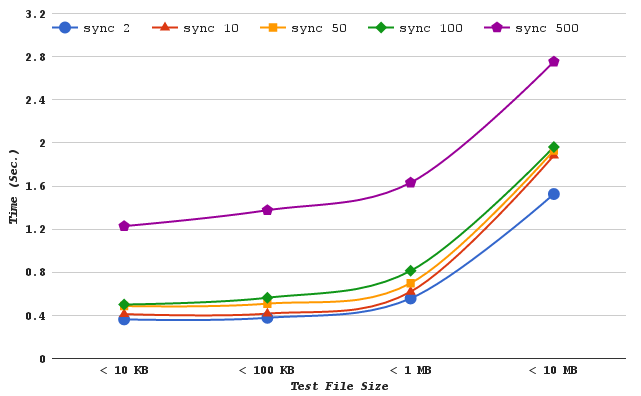
\includegraphics[width=.6\textwidth]{2014_upload_not_same}
    \end{center}
\end{frame}

\begin{frame}{Experimental Results}
{The client device and SP are \alert{not} in the same network segment - 2014 Cloud Com}
	\scriptsize
    \begin{table}[]
    \centering
    \caption{THE EXECUTION TIME OF \alert{DOWNLOAD} OPERATIONS (IN SEC.) (Account C)}
    \begin{tabular}{lccccl}
                         & sync 2   & sync 10  & sync 50  & sync 100 & sync 500  \\ \hline
        \textless 10 KB  & 0.388 & 0.374 & 0.524 & 0.646 & 2.269  \\ \hline
        \textless 100 KB & 0.427 & 0.440 & 0.584 & 0.735 & 2.302  \\ \hline
        \textless 1 MB   & 0.574 & 0.687 & 0.772 & 0.914 & 2.519  \\ \hline
        \textless 10 MB  & 0.933 & 1.024 & 1.145 & 1.414 & 2.884  \\ \hline
    \end{tabular}
    \end{table}
    \begin{center}
		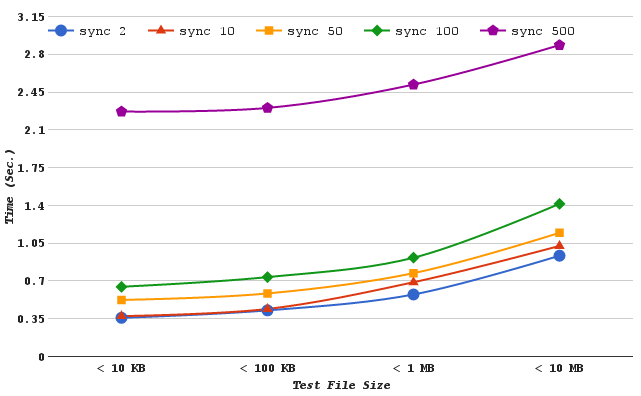
\includegraphics[width=.6\textwidth]{2014_download_not_same}
    \end{center}
\end{frame}

\begin{frame}{Experimental Results}
{The client device and SP are \alert{not} in the same network segment - UPLOAD operation}
	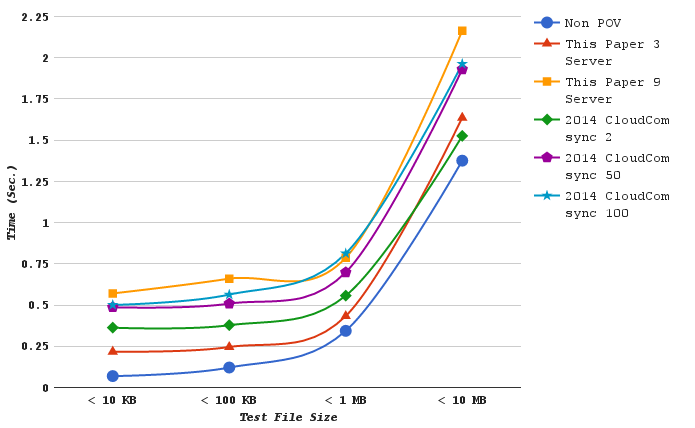
\includegraphics[width=\textwidth]{all_upload_not_same}
\end{frame}

\begin{frame}{Experimental Results}
{The client device and SP are \alert{not} in the same network segment - DOWNLOAD operation}
	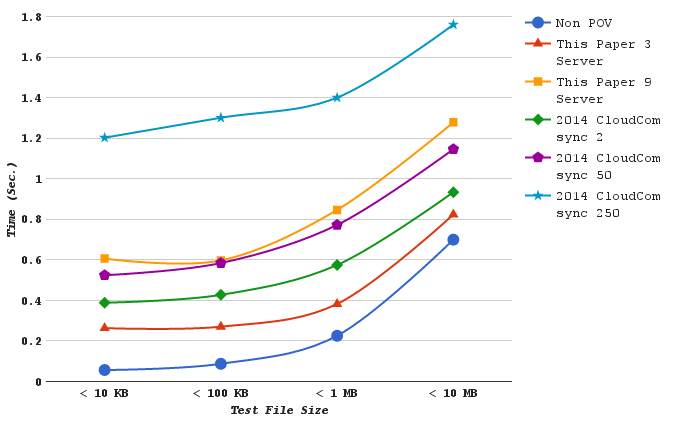
\includegraphics[width=\textwidth]{all_download_not_same}
\end{frame}

%TIMES
\begin{frame}{Experimental Results}
{The client device and SP are \alert{not} in the same network segment - UPLOAD Overhead}
	\scriptsize
    \begin{table}[]
    \centering
    \caption{My Method / Non POV (IN SEC.) (Account C)}
    \begin{tabular}{lcccc}
                         & 3 Server & 5 Server & 7 Server & 9 Server \\ \hline
        \textless 10 KB  & 3.14 & 4.78 & 6.73 & 8.23 \\ \hline
        \textless 100 KB & 2.02 & 3.38 & 3.95 & 5.45 \\ \hline
        \textless 1 MB   & 1.26 & 1.73 & 1.86 & 2.28 \\ \hline
        \textless 10 MB  & 1.18 & 1.43 & 1.46 & 1.57 \\ \hline
    \end{tabular}
    \caption{2014 Cloud Com / Non POV (IN SEC.) (Account C)}
    \begin{tabular}{lccccl}
                         & sync 2   & sync 10  & sync 50  & sync 100 & sync 500 \\ \hline
        \textless 10 KB  & 5.23 & 5.94 & 7.02 & 7.22   & 17.72  \\ \hline
        \textless 100 KB & 3.11 & 3.43 & 4.20 & 4.65   & 11.35  \\ \hline
        \textless 1 MB   & 1.62 & 1.80 & 2.03 & 2.36   & 4.74   \\ \hline
        \textless 10 MB  & 1.10 & 1.36 & 1.40 & 1.42   & 2.00   \\ \hline
    \end{tabular}
    ~\\
    ~\\
    ~\\
    \alert{Avg: 1.42 times, Max: 2.15 times}
    \end{table}
\end{frame}

\begin{frame}{Experimental Results}
{The client device and SP are \alert{not} in the same network segment - DOWNLOAD Overhead}
	\scriptsize
    \begin{table}[]
    \centering
    \caption{My Method / Non POV (IN SEC.) (Account C)}
    \begin{tabular}{lcccc}
                         & 3 Server & 5 Server & 7 Server & 9 Server \\ \hline
        \textless 10 KB  & 4.65 & 6.32 & 8.65 & 9.82 \\ \hline
        \textless 100 KB & 3.09 & 4.53 & 6.49 & 6.83 \\ \hline
        \textless 1 MB   & 1.69 & 2.62 & 3.07 & 3.75 \\ \hline
        \textless 10 MB  & 1.17 & 1.55 & 1.72 & 1.82 \\ \hline
    \end{tabular}
    \caption{2014 Cloud Com / Non POV (IN SEC.) (Account C)}
    \begin{tabular}{lccccl}
                         & sync 2   & sync 10  & sync 50  & sync 100 & sync 500 \\ \hline
        \textless 10 KB  & 6.86 & 6.60 & 9.25 & 11.41  & 40.07  \\ \hline
        \textless 100 KB & 4.89 & 5.04 & 6.68 & 8.41   & 26.36  \\ \hline
        \textless 1 MB   & 2.54 & 3.04 & 3.42 & 4.05   & 11.16  \\ \hline
        \textless 10 MB  & 1.33 & 1.46 & 1.63 & 2.02   & 4.12   \\ \hline
    \end{tabular}
    ~\\
    ~\\
    ~\\
    \alert{Avg: 1.88 times, Max: 4.08 times}
    \end{table}
\end{frame}